\documentclass[../main.tex]{subfiles}
\graphicspath{{\subfix{../imgs/}}}
\begin{document}

\chapter{Introducción} \label{cap:intro}
Este trabajo propone el diseño e implementación de un sistema para la programación y navegación de robots aéreos. El diseño persigue una estructura modular donde los diferentes bloques que constituyen el sistema puedan sustituirse para adaptarlos al problema, y que a su vez, permita la reutilización del código en diversas circunstancias.

Este primer capítulo recoge una introducción a la materia de estudio, la robótica aérea. Además, se expone la motivación cuyo resultado ha derivado en este trabajo, junto al problema concreto al cual se  pretende dar solución y los objetivos extraídos del problema.

\section{Robótica aérea} \label{section:intro-contexto}
El término \emph{robot} aparece por primera vez en 1920, en la obra teatral \emph{Rosum's Universal Robots} del escritor checo Karel Capek en cuyo idioma la palabra ``robota'' significa fuerza o servidumbre \cite{martin2007historia}. El nacimiento de la robótica y los robots surge asociado a la idea de trabajo y producción tras la Segunda Revolución Industrial y a lo largo del siglo XX. La automatización industrial de aquella época da lugar a los primeros sistemas de control automático que se extienden rápidamente a todos los sectores industriales, y que dan lugar a la robótica industrial tal como la conocemos hoy en día \cite{baturone2005robotica}.

El término \emph{robótica} es acuñado por Isaac Asimov, definiendo a la ciencia que estudia a los robots. El propio Asimov postuló también las Tres Leyes de la Robótica en su libro \emph{Yo Robot} publicado en 1950 \cite{martin2007historia}. El término ha evolucionado mucho desde sus inicios, hoy entendemos la robótica como la rama de la tecnología que estudia el diseño y construcción de máquinas capaces de desempeñar tareas realizadas por el ser humano o que requieren el uso de inteligencia \cite{rae}. Como se puede entender, la visión actual es mucho más amplia que en sus inicios y abarca muchas áreas de la ingeniería.

Existen diversas clasificaciones de los robots en función de su arquitectura, de su aplicación, de su cronología, etc. Una de estas clasificaciones distingue robots en función de su morfología \cite{de2006robotica}, que suele distinguir los siguientes tipos:

\begin{itemize}
    \item \textbf{Poliarticulados:} Son artilugios mecánicos y electrónicos destinados a realizar de forma automática determinados procesos de fabricación o manipulación. Suelen ser fijos, aunque también pueden realizar desplazamientos limitados y poseen un espacio de trabajo concreto y limitado. Los mejores ejemplos son los robots industriales, manipuladores o cartesianos.
    \item \textbf{Móviles:} Están provistos de algún tipo de mecanismo que les permite desplazarse autónomamente, como patas o ruedas, y reciben información de su entorno a través de sus propios sensores. Son ampliamente utilizados en el transporte de mercancías o en la exploración de lugares de difícil acceso. Pueden ser terrestres, acuáticos, aéreos o espaciales.
    \item \textbf{Androides:} Intentan reproducir total o parcialmente la forma y el comportamiento del ser humano. No solo imitan la apariencia humana (antropomorfismo), si no que emulan también la conducta de forma autónoma.
    \item \textbf{Zoomórficos:} Son aquellos que trata de reproducir en mayor o menor grado de realismo los sistemas de locomoción de diversos seres vivos. Este tipo podría incluir también a la morfología androide, en función del autor de la clasificación. Una subclasificación distingue entre robots caminadores y no caminadores.
\end{itemize}

Además de la robótica industrial, la otra gran rama de esta ciencia es la robótica de servicios. Actualmente este se encuentra en gran crecimiento a medida que aplicaciones útiles se pueden abordar con robots, ya lejos de las factorías. Es el caso de los robots de limpieza, los coches autónomos, los robots médicos o los robots aéreos.

La robótica aérea es la rama de la robótica que se encarga del estudio del comportamiento autónomo de aeronaves no tripuladas. Se entiende como una aeronave no tripulada (UAV, \emph{Unmanned Aerial Vehicle}, o más recientemente UAS, \emph{Unmanned Aircraft System}) a aquella que es capaz de realizar una misión sin necesidad de tener una tripulación embarcada \cite{barrientos2007vehiculos}. Otro término que también se utiliza con frecuencia es VANT, Vehículo Aéreo No Tripulado. A lo largo de esta memoria se utilizará el término \emph{drones} en referencia a este tipo de sistemas, cuyo uso está muy extendido. \\

\begin{figure}[!h]
 	\ffigbox[\FBwidth]{
 	    \caption[Clasificación de UAVs]{Clasificación de UAVs \cite{barrientos2007vehiculos}.}
        \label{fig:clasif-uav}
 	}
 	{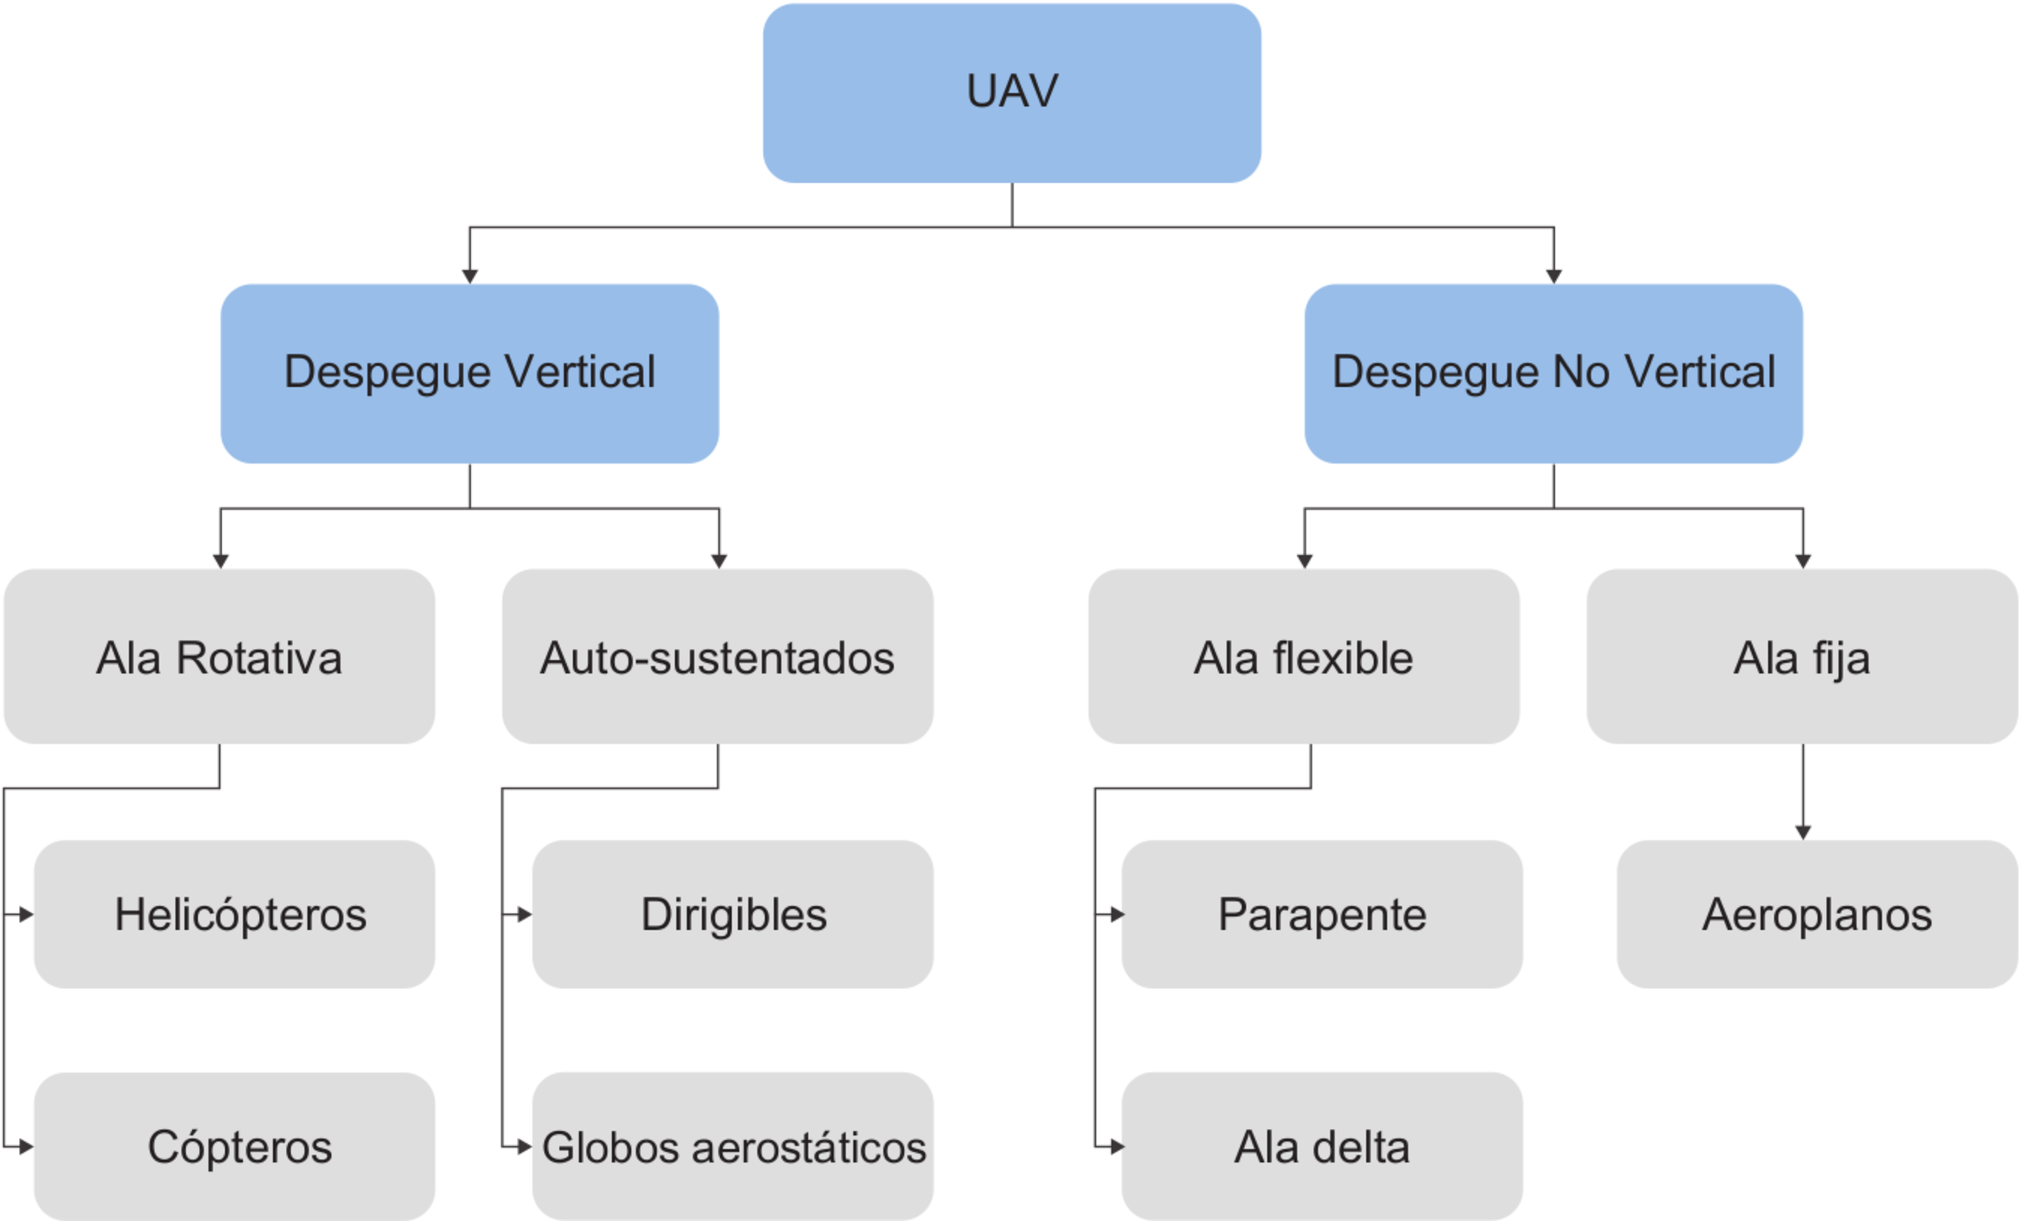
\includegraphics[width=0.9\textwidth]{01/fig_tipos_auv.pdf}}
\end{figure}

\newpage
A la hora de establecer una clasificación de los UAV es posible atender a diferentes criterios. Siguiendo la clasificación propuesta por Barrientos et al. \cite{barrientos2007vehiculos} se distinguen aeronaves en función del tipo de despegue, que puede ser vertical o no. A su vez, podemos subdividir las aeronaves en función del origen de su sustentación o del tipo de ala que poseen. Esta clasificación se representa en la Figura \ref{fig:clasif-uav}, mientras que en la Figura \ref{fig:ejemp-uav} se muestran dos ejemplos de diferentes tipos de UAV.

\begin{figure}[ht]
 	\ffigbox[\FBwidth]{
        \begin{subfigure}{0.45\textwidth}
            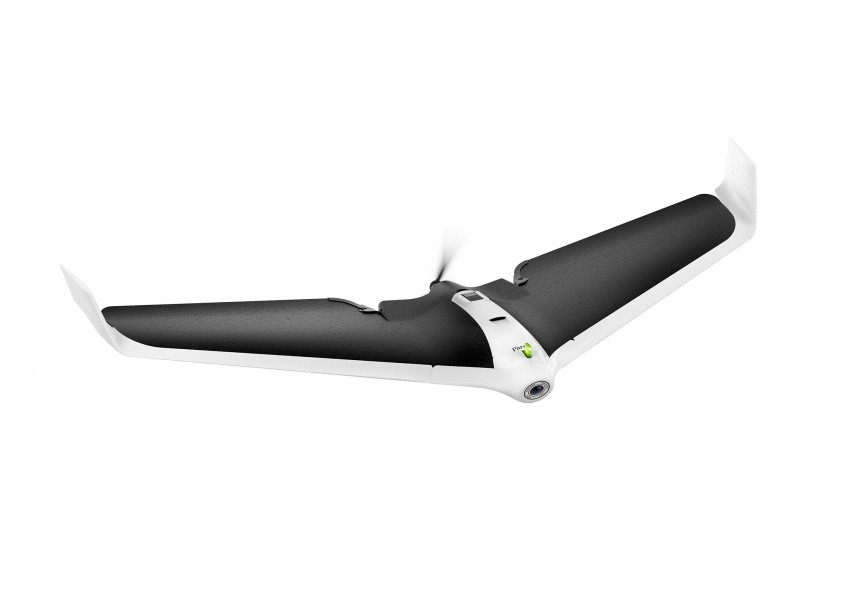
\includegraphics[height=4cm]{01/alafija.jpeg}
            \caption[Aeroplano]{Aeroplano.}
            \label{fig:tipo1}
        \end{subfigure}
        \begin{subfigure}{0.45\textwidth}
            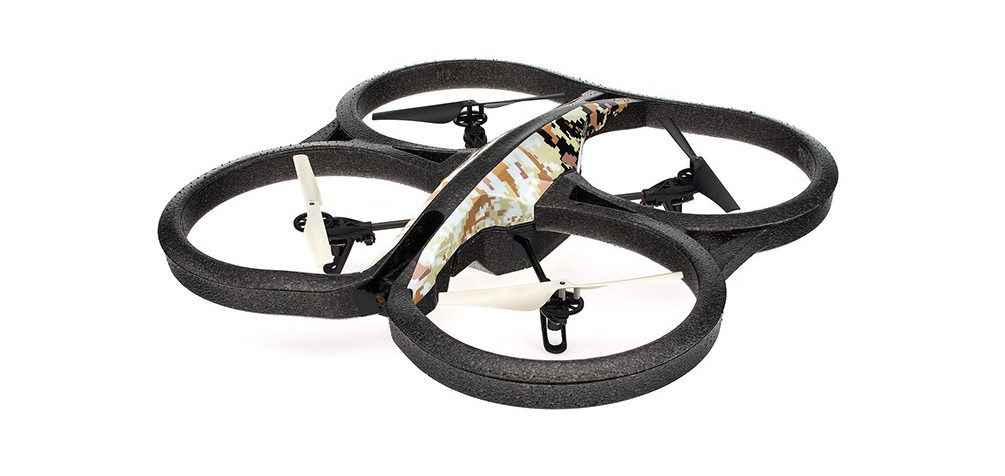
\includegraphics[height=3.75cm]{01/coptero.jpeg}
            \caption[Multicóptero]{Multicóptero.}
            \label{fig:tipo2}
        \end{subfigure}
 	}{
 	    \caption[Ejemplos de UAVs]{Ejemplos de UAVs.}
 	    \label{fig:ejemp-uav}
 	}
\end{figure}

Otros criterios de clasificación pueden responder a las capacidades de vuelo como el alcance, la altitud, la autonomía o la carga máxima. A su vez, también se pueden clasificar las aeronaves en función de la actividad que realizan. Algunas de estas clasificaciones distinguen entre uso civil y militar o aplicaciones en explotación (producto) o en desarrollo (prototipo). \\
Entre las principales aplicaciones civiles donde se emplean drones se encuentran el transporte, tanto de mercancías (ver Fig. \ref{fig:amazon}) como de personas, la seguridad y/o vigilancia (Fig. \ref{fig:dgt-drone}), la pesca y agricultura, la cartografía o el ocio y entretenimiento, entre otros.

\begin{figure}[ht]
 	\ffigbox[\FBwidth]{
 	    \caption[Aeronave de vigilancia en carretera perteneciente a la DGT]{Aeronave de vigilancia en carretera perteneciente a la Dirección General de Tráfico \cite{dgt-2021}.}
        \label{fig:dgt-drone}
 	}
 	{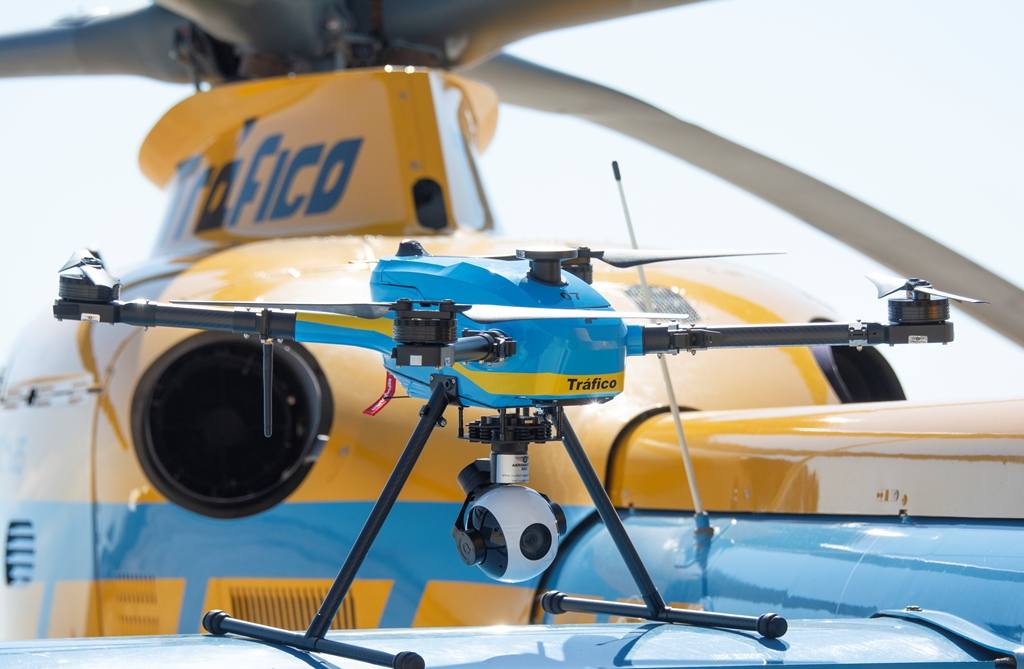
\includegraphics[width=0.79\textwidth]{01/mir_presentacion_drones_DGT.jpg}}
\end{figure}

\begin{figure}[ht]
 	\ffigbox[\FBwidth]{
 	    \caption[Aeronave de paquetería de Amazon]{Aeronave de paquetería de Amazon \cite{amazon}.}
        \label{fig:amazon}
 	}
 	{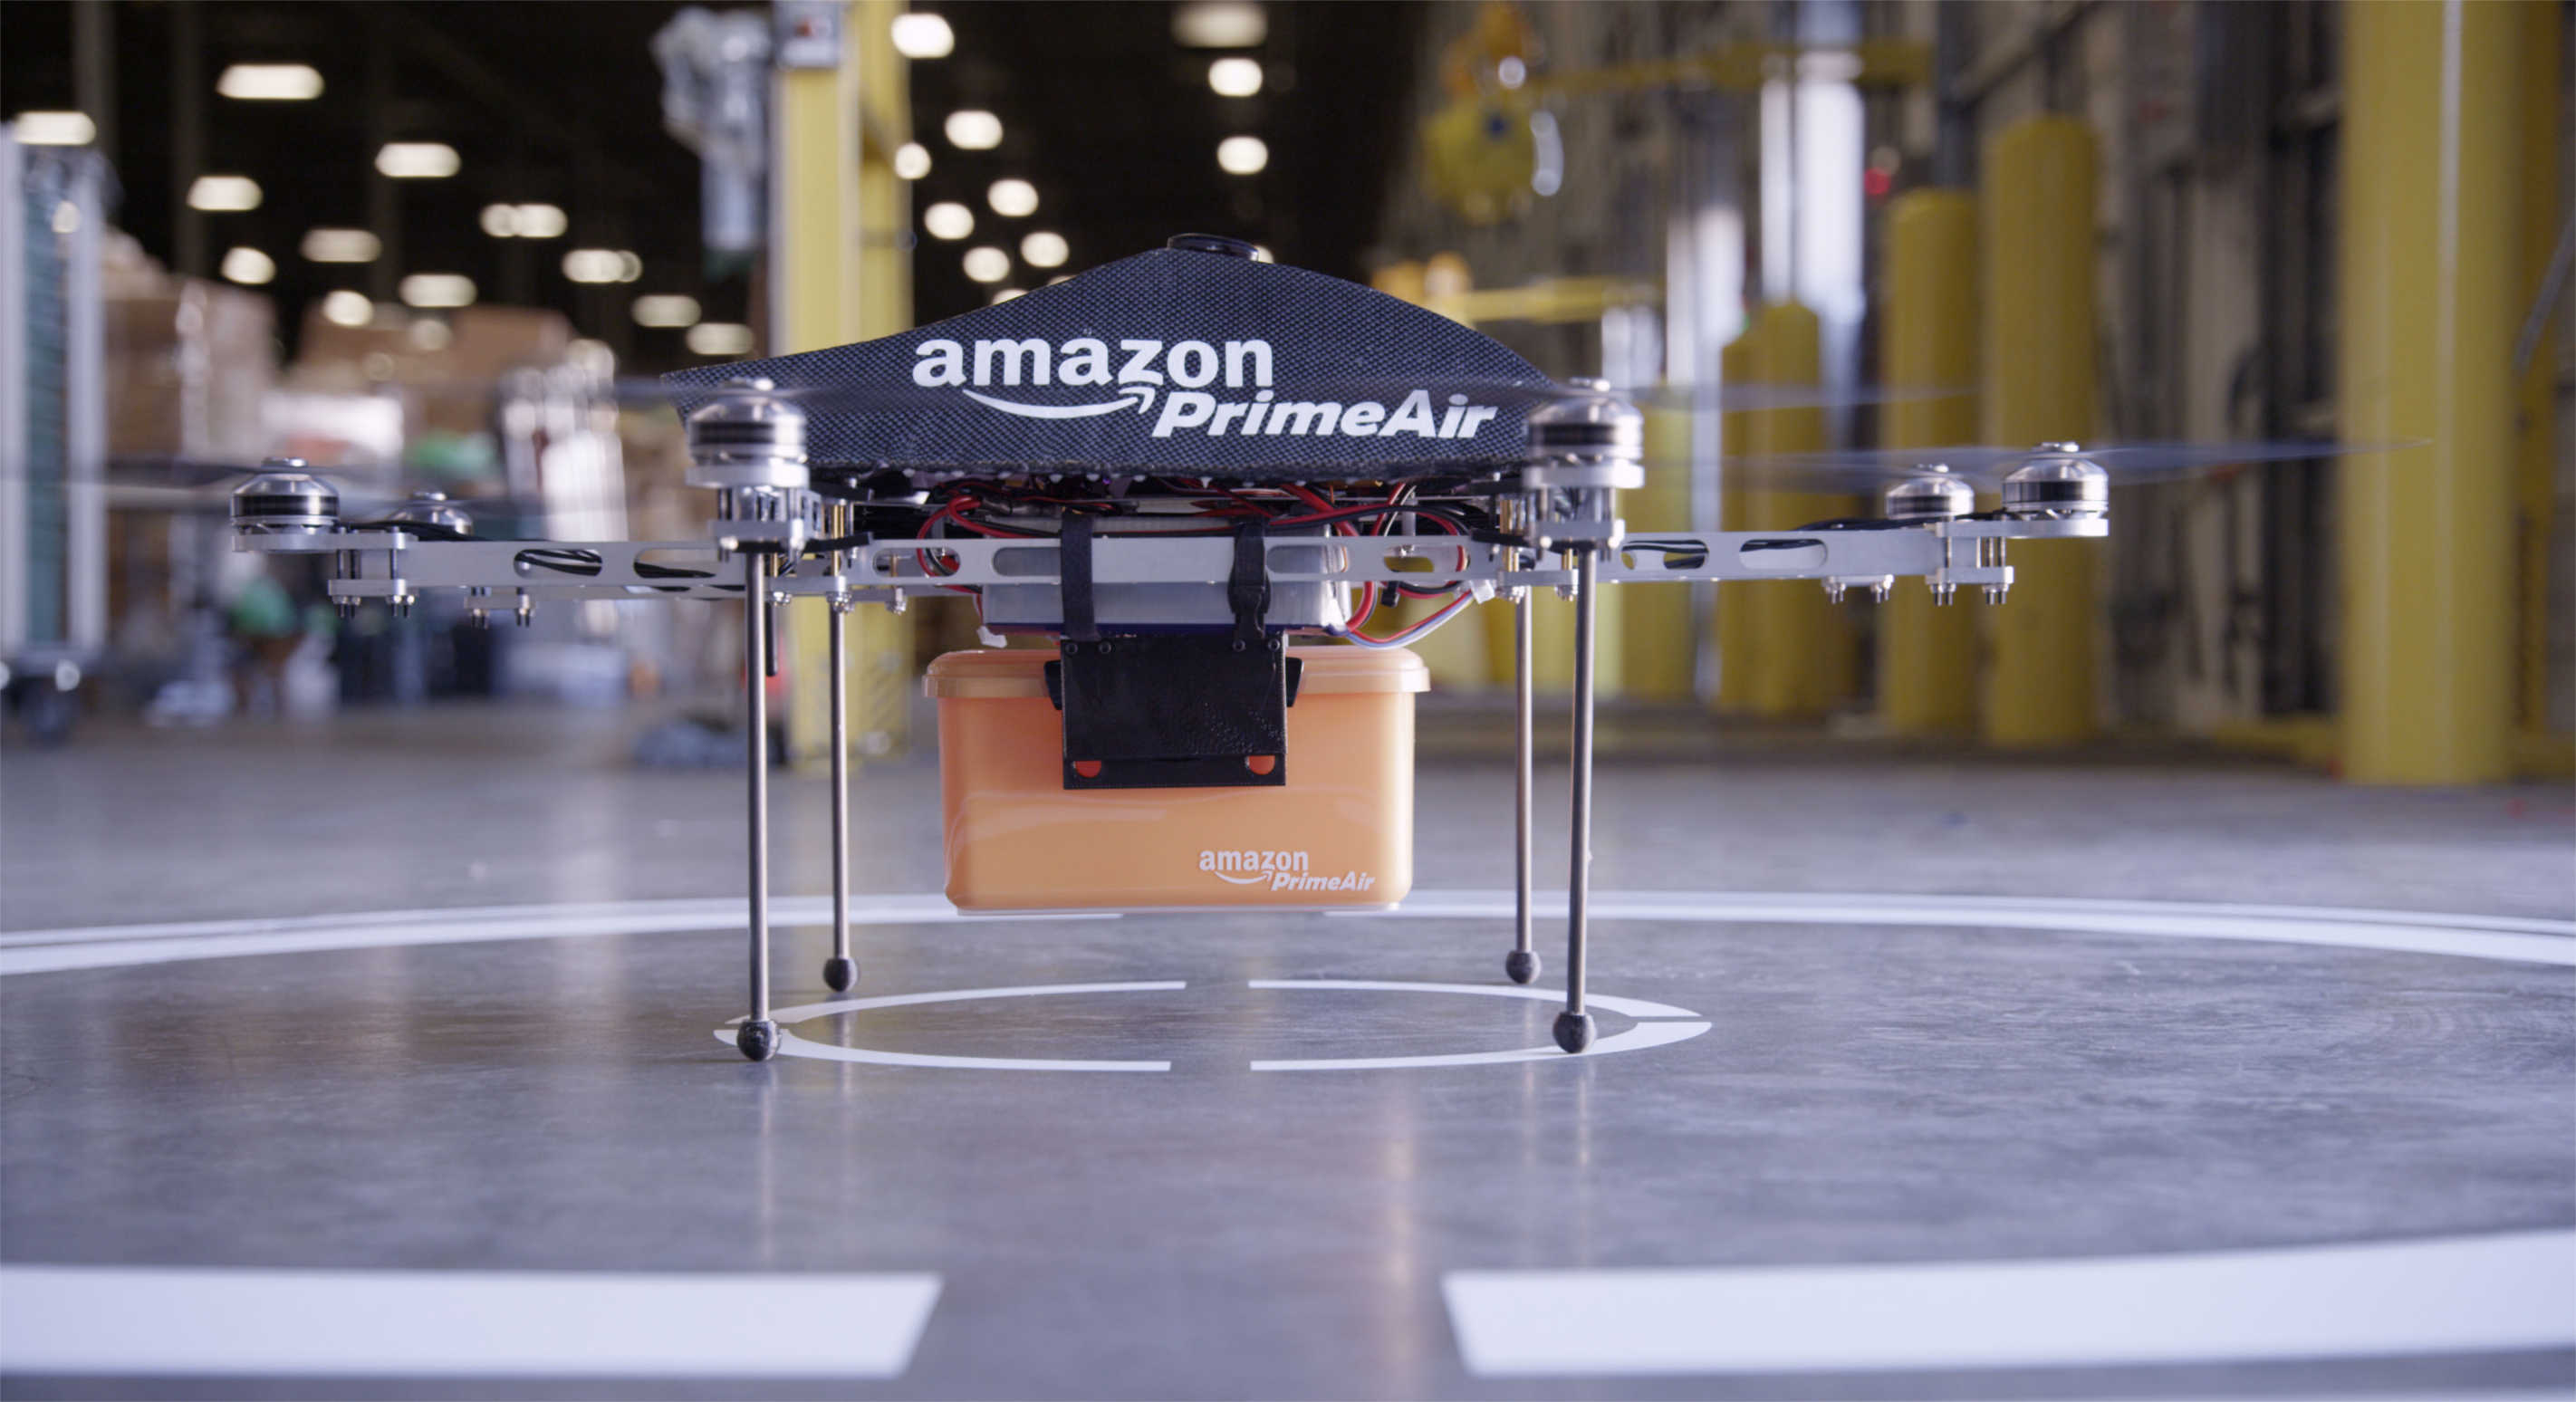
\includegraphics[width=0.79\textwidth]{01/prime-air.jpg}}
\end{figure}

% Amazon prime video
% 

% https://www.amazon.com/Amazon-Prime-Air/b?node=8037720011
%     \begin{subfigure}{0.5\textwidth}
%         \includegraphics[height=6cm, width=0.9\linewidth]{transporte.jpg}
%         \caption{Transporte de mercancías \cite{tfg-diego}.}
%         \label{fig:aplic1}
%     \end{subfigure}
%     \begin{subfigure}{0.5\textwidth}
%         \includegraphics[height=6cm, width=0.9\linewidth]{entretenimiento.jpg}
%         \caption{Spot publicitario \cite{tfg-jorge}.}
%         \label{fig:aplic2}
%     \end{subfigure}
        
%     \begin{subfigure}{0.5\textwidth}
%         \includegraphics[height=6cm, width=0.9\linewidth]{agricultura.jpg}
%         \caption{Agricultura \cite{tfg-jorge}.}
%         \label{fig:aplic3}
%     \end{subfigure}
%     \begin{subfigure}{0.5\textwidth}
%         \includegraphics[height=6cm, width=0.9\linewidth]{salvamento.jpg}
%         \caption{Salvamento \cite{tfg-diego}.}
%         \label{fig:aplic4}
%     \end{subfigure}
     
%     \caption{Ejemplo de aplicaciones en robótica aérea.}
%     \label{fig:aplic-uav}
% \end{figure}

En la actualidad tiende a utilizarse el concepto de UAS frente al de UAV. La extensión del concepto de vehículo a sistema refleja que el vehículo aéreo autónomo precisa para su funcionamiento de todo un sistema y no solo de la aeronave instrumentada.

Típicamente, un sistema UAS se compone de el segmento aire, compuesto principalmente por la aeronave, y por el segmento tierra, compuesto por un computador donde se ejecuta algún software de control, habitualmente una estación terrestre. Entre ambos segmentos debe existir en todo momento una comunicación, que se realiza a través de un protocolo de comunicaciones. \\
Sin embargo, es posible prescindir del segmento tierra dotando de la suficiente inteligencia a la aeronave. La inmensa mayoría de los sistemas que hoy en día entendemos como \emph{inteligentes} o \emph{autónomos} llevan embarcado un ordenador con un software que les permite suprimir al segmento tierra de la ecuación. La complejidad del ordenador embarcado y del software de control marcará el nivel de \emph{inteligencia} de la aeronave y la necesidad, o no necesidad, del segmento tierra. \\
Embarcar el segmento tierra abordo de la aeronave supone un aumento en la complejidad del sistema, por lo que puede no ser siempre interesante. Las características de la plataforma aérea y el problema a resolver definirán si es necesario embarcar o no el software de control sobre la aeronave.

% Aplicaciones: producto vs prototipo
% Topografía, logística, inspección visual (vslam)

Actualmente la robótica aérea se encuentra en un alto nivel de maduración en Europa. Desde el año 2021, la Agencia Estatal de Seguridad Aérea (AESA) dispone que todo tipo de UAS debe seguir la normativa europea \cite{normativa}, independientemente de su tamaño o peso. Entre las nuevas medidas se encuentran que todo operador debe poseer de una licencia (número de operador) y disponer de un seguro de responsabilidad civil a terceros obligatorio, sean las intenciones con fines recreativos o comerciales. Se puede obtener más información de la situación actual en el Reglamento de Ejecución (UE) 2019/947 \cite{regl-ejec} y en Reglamento Delegado (UE) 2019/945 \cite{regl-deleg} del Espacio Económico Europeo (EEA, \emph{European Economic Area}).

\section{Motivación} \label{section:intro-motivacion}
El ámbito de la robótica y de los vehículos aéreos no tripulados es un sector caracterizado por una fuerte expansión en los últimos tiempos, con unas expectativas de crecimiento y de demanda de personal cualificado tanto a nivel europeo como nacional muy relevantes para los próximos años. En el año 2035 el volumen de negocio anual estimado será 10.000M€ y 90.000 puestos de trabajo (1.220M€ y 11.000 ud solo para España), pasando en el año 2050 a un volumen de 14.600M€ y 110.000 puestos de trabajo (1.520M€ y 11.500 ud caso español) \cite{fomento-2018}.

\begin{figure}[ht]
 	\ffigbox[\FBwidth]{
 	    \caption[Evolución del número de modelos de drones según su ámbito de aplicación a nivel mundial]{Evolución del número de modelos de drones según su ámbito de aplicación a nivel mundial \cite{fomento-2018}.}
        \label{fig:uso-uavs}
 	}
 	{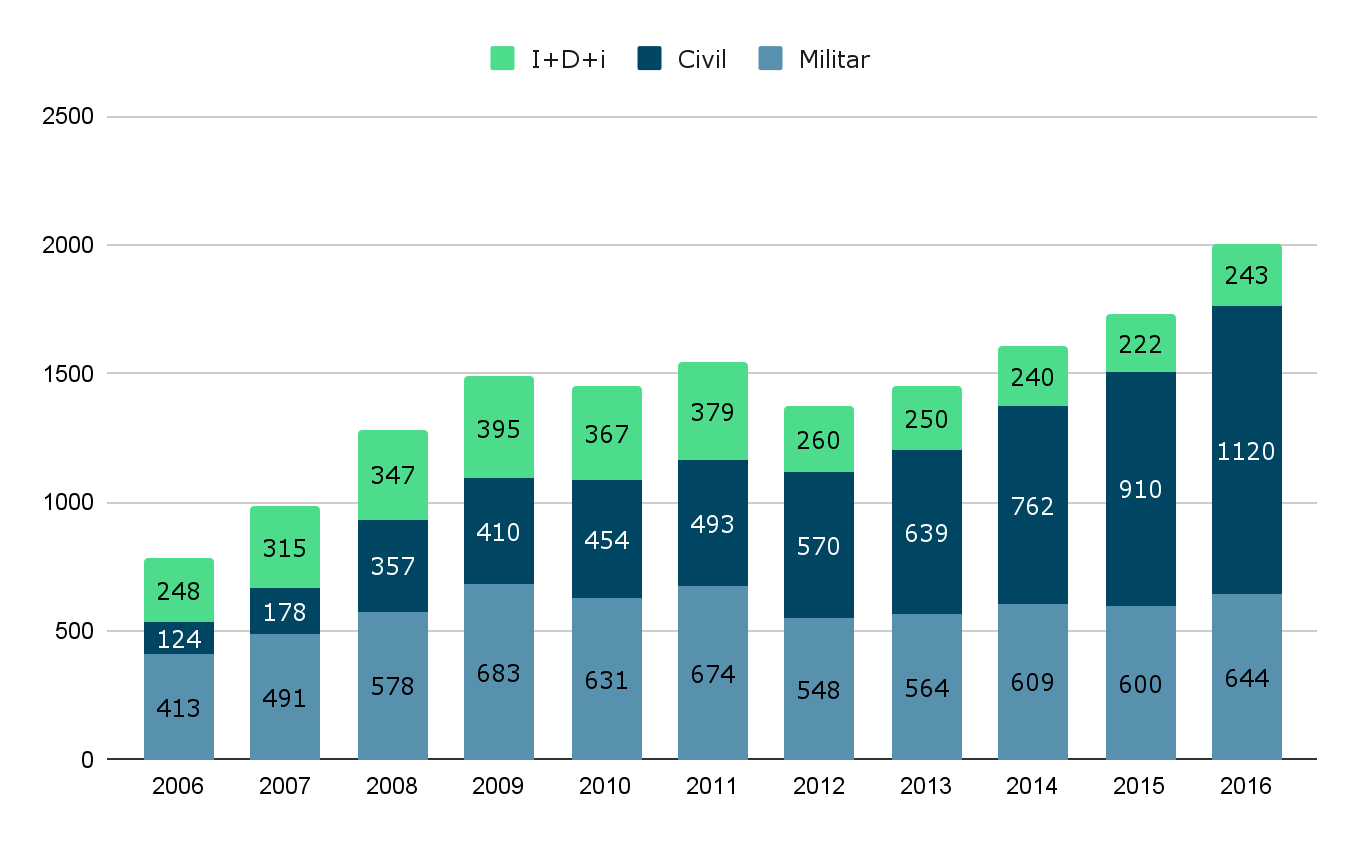
\includegraphics[width=0.9\textwidth]{01/uso-uavs.png}}
\end{figure}

La importancia del vuelo autónomo se ha visto reflejada en el alto incremento del uso de UAVs (ver Fig. \ref{fig:uso-uavs}).
Recientemente, los UAV se utilizan ampliamente tanto en aplicaciones militares como civiles debido a su pequeño tamaño y gran capacidad de maniobra \cite{kim2019unmanned}. Especialmente en aplicaciones civiles, los usos de los UAV se han expandido a casi todas las áreas. En el área de la agricultura, la rápida evolución de los UAV puede conducir a aplicaciones de agricultura de precisión, como la monitorización aérea de cultivos y las tareas de fumigación inteligente \cite{radoglou2020compilation}. En el campo industrial, los desarrollos de los UAV mejoran la eficiencia de misiones como inspección industrial (e.g. plantas fotovoltaicas) \cite{yao2019unmanned}, identificación de carga y entrega o logística, fuertemente ligadas a técnicas de \emph{slam} visual (VSLAM). Además, los UAV también se pueden ver en tareas de búsqueda y rescate, de topografía o de vigilancia entre otras aplicaciones.

La revolución en la robótica aérea también ha supuesto un gran avance en la normativa legal europea y nacional, donde Europa se aproxima al futuro \emph{U-Space}, un conjunto de nuevos servicios y procedimientos específicos diseñados para respaldar el acceso seguro, eficiente y protegido al espacio aéreo para un gran número de drones \cite{u-space}. \\
El proyecto \emph{U-Space} es promovido por la institución europea SESAR (\emph{Single European Sky ATM Research}) que se encarga del diseño del cielo único europeo y su gestión del tráfico aéreo (ATM, \emph{Air Traffic Management}) de forma común por los estados miembros de Unión Europea. Espacio aéreo que compartirán de forma habitual aeronaves tripuladas y UAS, bajo una gestión del tráfico común. \\
A mayores, la normativa legal vigente se encuentra en continua evolución para permitir nuevas aplicaciones manteniendo la seguridad existente, como ha ocurrido este último año en el ámbito europeo con la nueva normativa europea de UAS \cite{normativa}.

Dentro del ámbito nacional, el Ministerio de Ciencia e Innovación recoge en el documento Estrategia Española de Ciencia, Tecnología e Innovación 2021-2027 \cite{eecti-2021} las Líneas Estratégicas de I+D+I nacional. Entre ellas se encuentra Inteligencia Artificial y Robótica, en el ámbito de intervención de Mundo Digital, Industria, Espacio y Defensa, ratificando la relevancia que están cobrando los UAVs en los últimos años.

Pese al gran avance tecnológico, el desarrollo de aplicaciones para UAS sigue siendo complejo. Este tipo sistemas son heterogéneos (plataformas de vuelo muy diferentes), con muchos ingredientes integrados (autopilotos, subsistemas de control y estabilización, de comunicaciones, de navegación, de percepción...) y en un escenario peligroso, donde un error puede suponer la caída de la aeronave o el daño a terceros.

Por ello, y debido a la gran expansión social y económica que está sufriendo esta materia, se observa que existe la necesidad de herramientas que permitan construir aplicaciones para el uso extendido de drones. Herramientas que permitan abstraerse de las complejidades que lleva asociada una aeronave e incluso de la plataforma en sí. \\
Este trabajo persigue ese fin. Busca proporcionar al usuario un entorno para la programación y navegación de robots aéreos, que permita al usuario centrar sus esfuerzos en resolver solamente la aplicación final del dron, y olvidarse del resto de complejidades.

\section{Problema} \label{section:intro-problema}
El problema a resolver es realmente complejo, alcanzar un software seguro y robusto que permita el vuelo autónomo de aeronaves es inabarcable en tiempo y esfuerzo para este trabajo. Por ello, este trabajo se centra en un subconjunto del problema. En concreto, se busca un software intermedio, a modo de \emph{middleware}, que permita conectar distintas plataformas de vuelo con diferentes aplicaciones finales, las cuales quedarían a cargo del desarrollo del usuario.
Se utiliza la palabra \emph{middleware}, ya que el software propuesto se encuentra a medio camino entre las aplicaciones (software) y las aeronaves (hardware). \\
Entras las aplicaciones posibles, la herramienta a desarrollar busca ofrecer soluciones para la creación de algoritmos de navegación autónomos. Más allá del típico control por posición en exteriores, basado en GPS, se persiguen aplicaciones basadas en posición en interiores (en ausencia de GPS), p.e. algoritmos de auto-localización visual (\emph{visual SLAM}), o aplicaciones de control visual, no basadas en posición.

Por último, con el propósito de acotar todavía más el problema, este trabajo solo se centrará en el uso de un tipo de aeronaves, los multicópteros, cuyo uso es el más extendido dentro de todos los tipos de aeronaves.

\section{Objetivos} \label{section:intro-objetivos}
Este trabajo presenta una serie de objetivos principales y secundarios. En primer lugar, se quiere desarrollar herramientas software que permitan la programación y navegación de multicópteros. Este primer objetivo se abordará creando una solución software que ofrezca al usuario una interfaz de programación de aplicaciones (API, \emph{Application Programming Interface}) que facilite el desarrollo de aplicaciones. \\
Asociado a este objetivo principal, se encuentran un grupo de características del código considerados como atributos de calidad y objetivos secundarios. Se precisa un software intuitivo y sencillo de usar (los usuarios no tienen por qué ser expertos en drones), robusto y seguro, al tratarse de un software que trabaja directamente con drones. Cabe destacar que estas aplicaciones pueden ser creadas por usuarios ajenos al resto del software e incluso a la aeronave utilizada. Además, el software que se propone está enfocado a un público, el cual, aunque sí deba tener unas nociones básicas en robótica, no tiene por qué ser experto en drones. Por tanto, se consideran como objetivos secundarios ligados a este primer objetivo principal la usabilidad, la seguridad y la robustez del código.

En segundo lugar, se pretende extender dicho software para el uso de diferentes plataformas aéreas. Así, otro de los objetivos principales del software es que sea multiplataforma y se pueda utilizar con diferentes aeronaves. Para ello, se realizarán diferentes pruebas que permitan comprobar el funcionamiento del software con varias aeronaves. \\
Como objetivo secundario ligado a este segundo objetivo, se buscará utilizar aeronaves de distinta naturaleza dentro de los multicópteros. Una variedad en las aeronaves usadas durante las pruebas dará una mejor perspectiva del alcance del trabajo realizado. Aunque durante el Capítulo  \ref{cap:herram} se profundizará sobre las herramientas disponibles para este trabajo, es necesario introducir las posibles alternativas existentes para el correcto entendimiento de los objetivos. Entre los multicópteros se distinguen aeronaves reales o simuladas, y orientadas a un vuelo en interiores o en exteriores.

En tercer lugar, se realizarán diferentes aplicaciones ilustrativas similares a las desarrolladas por los futuros usuarios. Dichas aplicaciones harán uso de la solución desarrollada para el primer objetivo del trabajo y se basarán en algún control reactivo visual. \\
Dichas aplicaciones tratarán de mostrar ejemplos de aplicaciones de dificultad variable, partiendo de un uso básico de las herramientas recogidas en este trabajo, hasta el desarrollo de algoritmos navegación basado en aprendizaje profundo.

Así pues, y a modo de resumen, los objetivos contemplados en este trabajo son:
\begin{enumerate}
    \item \textbf{Desarrollo de herramientas para la programación y navegación de multicópteros.} El diseño se centrará en la usabilidad, la seguridad y robustez del software.
    \item \textbf{Comprobaciones sobre distintas plataformas aéreas.} Multicópteros de diversa índole, haciendo uso de aeronaves reales, simuladas, de interiores y de exteriores.
    \item \textbf{Desarrollo de diferentes aplicaciones de control.} Aplicaciones de distinto nivel de dificultad técnica, partiendo de usos básicos centrados en navegación hasta algoritmos complejos basados en aprendizaje profundo.
\end{enumerate}

\section{Estructura de la memoria} \label{section:intro-estructura}
Esta última sección describe la estructura de la memoria, introduce los diferentes capítulos y los temas que se tratarán en cada uno de los mismos.

En primer lugar se encuentra este capítulo introductorio (Cap. \ref{cap:intro}) que se concibe como una serie de aclaraciones previas y necesarias para el correcto entendimiento del trabajo en su conjunto. Incluye un contexto histórico de la robótica, la robótica aérea y las estaciones de tierra y sus aplicaciones, que establecen el marco en el que se sitúa este trabajo. A continuación incluye el problema abordado en este trabajo y la motivación del mismo, es decir, ¿qué se trata de resolver con este trabajo?, y ¿por qué surge la necesidad del mismo?. Se incluyen también los objetivos principales y secundarios que ha de cumplir la solución desarrollada.

En el Capítulo \ref{cap:herram} se detallan las herramientas software y hardware que constituyen el estado del arte, ofreciendo una visión global de la robótica aérea actual. Para ello, se realiza un pequeño estudio de las principales herramientas presentes tanto en la comunidad científica como en la industria. \\
Además, este capítulo recoge en diferentes secciones cada uno de los elementos que entran en juego en un sistema aéreo. Por un lado, en una primera sección se explica el segmento tierra y su composición. Por otro lado, en la siguiente sección se detalla el segmento aire y sus componentes. Finalmente, el capítulo se centra en el protocolo de comunicaciones entre ambos lados, tierra y aire.

En el Capítulo \ref{cap:met} se presentan el material y método utilizados en este trabajo. Este capítulo recopila, de entre todas las herramientas existentes, los componentes concretos seleccionados para la resolución del problema. Además, ofrece una descripción pormenorizada de los mismos, junto con la motivación de su elección. 

En el Capítulo \ref{cap:infra} se explica la infraestructura software desarrollada para dar solución al problema. En una primera sección se explica detalladamente el diseño elegido y se explican también varias decisiones relevantes a la hora de seleccionar el diseño. En la secciones sucesiva se describe la implementación de cada una de las herramientas de código identificadas. 

En el Capítulo \ref{cap:aplic} se desarrollan las aplicaciones propuestas que permiten validar la solución presentada en el anterior capítulo. A lo largo del capítulo, se introducen las diferentes aplicaciones, se explican cada uno de los diseños y sus implementaciones y se presentan los resultados obtenidos tras el desarrollo en forma de diversos ensayos experimentales con pruebas de vuelo en simulación y en real.

Por último, en el Capítulo \ref{cap:concl} se recogen las conclusiones extraídas con la finalización del trabajo y se evalúan los distintos objetivos iniciales propuestos. A mayores, se exponen una serie de posibles vías de desarrollo futuro y de mejoras para la herramienta.

\end{document}